% **************************************************************************************************
% ** SPSC Report and Thesis Template
% **************************************************************************************************
%
% ***** Authors *****
% Daniel Arnitz, Paul Meissner, Stefan Petrik
% Signal Processing and Speech Communication Laboratory (SPSC)
% Graz University of Technology (TU Graz), Austria
%
% ***** Changelog *****
% 0.1   2010-01-25   extracted from report template by Daniel Arnitz (not ready yet)
% 0.2   2010-02-08   added thesis titlepage and modified layout (not ready yet)
% 0.3   2010-02-18   added TUG logo and statutory declaration
% 0.4   2010-02-18   moved the information fields below \input{./base/packages} (encoding...)
% 0.5   2010-03-02   added \ShortTitle to fix problems with long thesis titles
%                    added \ThesisType (makes the template suitable for MSc, BSc, PhD, ... Thesis)
% 0.6   2010-06-05   added pagestyle and pagenumbering after frontmatter, packages has now type
% 0.7   2010-09      \Advisors -> \Assessors, inserted frontmatter for thesis
% 0.8   2010-11      added examples
% 0.9   2011-04      \Twosided now {true,false}, scrbook for thesis (\front-, \main-, \backmatter)
%                    added \SpecialNote for titlepage (funding, etc.), added type "homework"
% 0.10  2011-10-18   fixed two typos in \bibliographystyle{} (bug reported by Michael Tauch)
% 0.11  2011-11-09   fixed/modified preamble (bug reported by Michael Tauch)
% 0.12  2012-07-20   added ./base/opt_macros to deal with optional macros
% 0.13  2012-07-27   added \PaperSize
%
% ***** Todo *****
% - Introduction/Usage
% - explain/show preamble (with \thispagestyle, etc)
% - why doesn't \pagestyle work in preamble while \thispagestyle does? (reported by Markus Fr�hle)
% **************************************************************************************************

% **************************************************************************************************
% basic setup
\newcommand{\DocumentType}{report} % "thesis" / "report" / "homework"
\newcommand{\DocumentLanguage}{en} % "en" / "de"
\newcommand{\PaperSize}{a4paper} % "a4paper" / "letterpaper"
\newcommand{\Twosided}{true} % "true" / "false"

% **************************************************************************************************
% template setup -- do not change these unless you know what you are doing!
\input{./base/packages_\DocumentType}
\input{./base/layout_\DocumentType}
% **************************************************************************************************
% ** SPSC Report and Thesis Template
% **************************************************************************************************
%
% ***** Authors *****
% Daniel Arnitz, Paul Meissner, Stefan Petrik
% Signal Processing and Speech Communication Laboratory (SPSC)
% Graz University of Technology (TU Graz), Austria
%
% ***** Changelog *****
% 0.1   2010-08-09   added \remc and \remq commands, \nxtpar now uses \med- instead of \bigskip
%                    replaced \lastfootnotemark by \oldfootnotemark (generalization),
%                    added \chapternote, set \openingquote to 0.4\textwidth, modified \MAttention,
%                    \xspace for marginpar commands, modified \MDanger and \MQuestion
% 0.2   2010-10-03   added \exp, colors "bk*"
% 0.3   2010-11-16   added \twofigs and \twofigsf
% 0.4   2010-12      added \F (Fourier), \ceil and \floor
% 0.5   2011-01      added chapter/section/figure/table/part reference commands, textrel
% 0.6   2011-03      added \avg, modified bkred, bkgreen, and bkblue colors,
%                    added \medskip to \chapternote, added natural/real/complex/... numbers
%                    added \rapp for references to the appendix
% 0.7   2011-04      removed labels from \new*NoTOC
% 0.8   2012-06      correction of minor typo
%
% ***** Todo *****
% ? prettyref instead of reference commands
%
% **************************************************************************************************



% **************************************************************************************************
% * SECTIONING AND TEXT
% **************************************************************************************************

% new chapter, section, ... plus a few addons
%   part
\newcommand{\newpart}[2]{\FloatBarrier\cleardoublepage\part{#1}\label{part:#2}}%
%   chapter
\newcommand{\newchapter}[2]{\FloatBarrier\chapter{#1}\label{chp:#2}}
\newcommand{\newchapterNoTOC}[1]{\FloatBarrier\stepcounter{chapter}\chapter*{#1}}%
%   section
\newcommand{\newsection}[2]{\FloatBarrier\vspace{5mm}\section{#1}\label{sec:#2}}%
\newcommand{\newsectionNoTOC}[1]{\FloatBarrier\vspace{5mm}\stepcounter{section}\section*{#1}}%
%   subsection
\newcommand{\newsubsection}[2]{\FloatBarrier\vspace{3mm}\subsection{#1}\label{sec:#2}}%
\newcommand{\newsubsectionNoTOC}[1]{\FloatBarrier\vspace{3mm}\stepcounter{subsection}\subsection*{#1}}%
%   subsubsection
\newcommand{\newsubsubsection}[2]{\vspace{2mm}\subsubsection{#1}\label{sec:#2}}%
\newcommand{\newsubsubsectionNoTOC}[1]{\vspace{2mm}\stepcounter{subsubsection}\subsubsection*{#1}}%

% references
%   chapter(s), section(s), appendix
\newcommand{\rchp}[1]{Chapter~\ref{chp:#1}}
\newcommand{\rchps}[1]{Chapters~\ref{chp:#1}}
\newcommand{\rsec}[1]{Section~\ref{sec:#1}}
\newcommand{\rsecs}[1]{Sections~\ref{sec:#1}}
\newcommand{\rappendix}[1]{Appendix~\ref{#1}}
%   figure(s), table(s), listing(s), equation(s)
\newcommand{\rfig}[1]{Fig.~\ref{fig:#1}}
\newcommand{\rfigs}[1]{Figs.~\ref{fig:#1}}
\newcommand{\rtab}[1]{Tab.~\ref{tab:#1}}
\newcommand{\rtabs}[1]{Tabs.~\ref{tab:#1}}
\newcommand{\rlst}[1]{Listing~\ref{lst:#1}}
\newcommand{\rlsts}[1]{Listings.~\ref{lst:#1}}
\newcommand{\req}[1]{(\ref{eq:#1})}

% varioref references
%   chapter(s), section(s)
\newcommand{\vrchp}[1]{Chapter~\vref{chp:#1}}
\newcommand{\vrchps}[1]{Chapters~\vref{chp:#1}}
\newcommand{\vrsec}[1]{Section~\vref{sec:#1}}
\newcommand{\vrsecs}[1]{Sections~\vref{sec:#1}}
%   figure(s), table(s), listing(s)
\newcommand{\vrfig}[1]{Fig.~\vref{fig:#1}}
\newcommand{\vrfigs}[1]{Figs.~\vref{fig:#1}}
\newcommand{\vrtab}[1]{Tab.~\vref{tab:#1}}
\newcommand{\vrtabs}[1]{Tabs.~\vref{tab:#1}}
\newcommand{\vrlst}[1]{Listing~\vref{lst:#1}}
\newcommand{\vrlsts}[1]{Listings~\vref{lst:#1}}

% next paragraph
\newcommand{\nxtpar}{\par\medskip}

% "stylish" quotes on the right side
\newcommand{\openingquote}[2]{\hfill\parbox[t]{0.4\textwidth}{\itshape\raggedleft{"#1"}\\\footnotesize -- #2}\nxtpar}%

% some information on the right side (sources, ...)
\newcommand{\chapternote}[1]{\vspace*{-\medskipamount}\hfill\parbox[t]{0.8\textwidth}{\itshape\footnotesize\raggedleft#1}\par\medskip}%

% direct quotes
% \newenvironment{directquote}{\nxtpar\hrule}{\hrule}\hfill\litref{#1}{#2}}

% warnings and attention signs in marginpar
\newcommand{\MDanger}{\marginpar{\raisebox{-2mm}{
\includegraphics[height=7mm]{base/MDanger}}}\xspace}%
\newcommand{\MAttention}{\marginpar{\raisebox{-2mm}{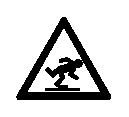
\includegraphics[height=7mm]{base/MAttention}}}\xspace}%
\newcommand{\MHint}{\marginpar{\raisebox{-2.25mm}{
\includegraphics[height=7mm]{base/MHint}}}\xspace}%
\newcommand{\MQuestion}{\marginpar{\raisebox{-2.25mm}{
\includegraphics[height=7mm]{base/MQuestion}}}\xspace}%

% same footnote number as last one
\newcommand{\oldfootnotemark}[1]{\addtocounter{footnote}{-#1}\footnotemark\addtocounter{footnote}{#1-1}}%
%\newcommand{\lastfootnotemark}{\addtocounter{footnote}{-1}\footnotemark}%

% value-unit commands (for 457 kHz, etc)
\newcommand{\vu}[2]{\mbox{\ensuremath{#1\,\text{#2}}}}% "value-unit" ... prevents e.g. 456 \linebreak mV
\newcommand{\vuc}[3]{\mbox{\ensuremath{#1\,\text{#2}\;#3\,\%}}} % "value~unit~tolerance-per-cent"
\newcommand{\vum}[3]{\mbox{\ensuremath{#1\,\text{#2}\;#3\,\perthousand}}} % "value~unit~tolerance-per-mil"

% reminders
\newcommand{\reminder}[1]{\colorbox{red}{#1}\xspace}%
\newcommand{\rem}{\reminder{(...)}}% shortcut for the full reminder
\newcommand{\remq}{\reminder{???}}% open question
\newcommand{\remc}{\reminder{[?]}}% open citation
\newcommand{\uc}{\nxtpar\colorbox{yellow}{... under construction ...}\nxtpar}%

% misc
\newcommand{\pwd}{.} % present working directory (can be used to create relativ paths per part, etc.)




% **************************************************************************************************
% * MATH
% **************************************************************************************************

% highlighting
\newcommand{\vm}[1]{\ensuremath{\bm{#1}}}% vector or matrix

% functions
\renewcommand{\exp}[1]{\ensuremath{\text{e}^{#1}}}% exponential
\renewcommand{\ln}[1]{\ensuremath{\text{ln}\!\left(#1\right)}}% natural logarithm
\newcommand{\ld}[1]{\ensuremath{\text{ld}\!\left(#1\right)}}% logarithm base 2
\renewcommand{\log}[1]{\ensuremath{\text{log}\!\left(#1\right)}}% logarithm (base 10)
\newcommand{\logb}[2]{\ensuremath{\text{log}_{#1}\!\left(#2\right)}}% logarithm base ...

% rounding
\newcommand{\round}[1]{\ensuremath{\text{round}\!\left(#1\right)}}% rounding towards next integer
\newcommand{\ceil}[1]{\ensuremath{\left\lceil#1\right\rceil}}% rounding towards infinity
\newcommand{\floor}[1]{\ensuremath{\left\lfloor#1\right\rfloor}}% rounding towards zero

% operators
\newcommand{\E}[1]{\ensuremath{\text{E}\!\left\{#1\right\}}}% expectation operator
\newcommand{\F}[1]{\ensuremath{\mathcal{F}\!\left\{#1\right\}}}% Fourier transform operator
\newcommand{\IF}[1]{\ensuremath{\mathcal{F}^{-1}\!\left\{#1\right\}}}% inverse Fourier transform operator
\newcommand{\var}[1]{\ensuremath{\text{var}\!\left\{#1\right\}}}% variance operator
\newcommand{\cov}[1]{\ensuremath{\text{cov}\!\left\{#1\right\}}}% covariance operator
\newcommand{\corr}[1]{\ensuremath{\text{corr}\!\left\{#1\right\}}}% correlation operator
\newcommand{\avg}[1]{\ensuremath{\text{avg}\!\left\{#1\right\}}}% averaging operator
\newcommand{\avgvar}[1]{\ensuremath{\overline{\text{var}}\!\left\{#1\right\}}}% average variance operator
\renewcommand{\Re}[1]{\ensuremath{\text{Re}\!\left\{#1\right\}}}% real part
\renewcommand{\Im}[1]{\ensuremath{\text{Im}\!\left\{#1\right\}}}% imaginary part

% numbers
\newcommand{\REAL}{\ensuremath{\mathbb{R}}}% real numbers
\newcommand{\NATURAL}{\ensuremath{\mathbb{N}}}% natural numbers
\newcommand{\INTEGER}{\ensuremath{\mathbb{Z}}}% integer numbers (natural numbers plus zero)
\newcommand{\COMPLEX}{\ensuremath{\mathbb{C}}}% complex numbers
\newcommand{\IMAG}{\ensuremath{\mathbb{I}}}% imaginary numbers

% other
\newcommand{\conj}{\ensuremath{^\ast}}% conjugate complex
\newcommand{\transp}{\ensuremath{^\text{T}}}% conjugate (Hermitian) transpose
\newcommand{\mtx}[2]{\left[\ensuremath{\begin{array}{#1}#2\end{array}\right]}}%vector/matrix
\newcommand{\isdef}{\ensuremath{\mathrel{:=}}}% definition left->right
\newcommand{\isdefflip}{\ensuremath{\mathrel{=:}}}% definition right->left
\newcommand{\isreq}{\ensuremath{\mathrel{\stackrel{!}{=}}}}% is required
\newcommand{\textrel}[1]{\ensuremath{{\;{#1}\;}}}% relation symbol for in-line equations (fixed spacing)



% **************************************************************************************************
% * FLOATS (FIGURES, TABLES, LISTINGS, ...)
% **************************************************************************************************

% figures without frames
%   standard
\newcommand{\fig}[3]{\begin{figure}\centering\includegraphics[width=\textwidth]{#1}\caption{#2}\label{fig:#3}\end{figure}}%
%   with controllable parameters
\newcommand{\figc}[4]{\begin{figure}\centering\includegraphics[#1]{#2}\caption{#3}\label{fig:#4}\end{figure}}%
%   two subfigures
\newcommand{\twofig}[6]{\begin{figure}\centering%
\subfigure[#2]{\includegraphics[width=0.495\textwidth]{#1}}%
\subfigure[#4]{\includegraphics[width=0.495\textwidth]{#3}}%
\caption{#5}\label{fig:#6}\end{figure}}%
%   two subfigures with labels for each subplot
\newcommand{\twofigs}[8]{\begin{figure}\centering%
\subfigure[#2]{\includegraphics[width=0.495\textwidth]{#1}\label{fig:#8#3}}%
\subfigure[#5]{\includegraphics[width=0.495\textwidth]{#4}\label{fig:#8#6}}%
\caption{#7}\label{fig:#8}\end{figure}}%
%   two subfigures and controllable parameters
\newcommand{\twofigc}[8]{\begin{figure}\centering%
\subfigure[#3]{\includegraphics[#1]{#2}}%
\subfigure[#6]{\includegraphics[#4]{#5}}%
\caption{#7}\label{fig:#8}\end{figure}}%

% framed figures
%   standard
\newcommand{\figf}[3]{\begin{figure}\centering\fbox{\includegraphics[width=\textwidth]{#1}}\caption{#2}\label{fig:#3}\end{figure}}%
%   with controllable parameters
\newcommand{\figcf}[4]{\begin{figure}\centering\fbox{\includegraphics[#1]{#2}}\caption{#3}\label{fig:#4}\end{figure}}%
%   two subfigures
\newcommand{\twofigf}[6]{\begin{figure}\centering%
\fbox{\subfigure[#2]{\includegraphics[width=0.495\textwidth]{#1}}}%
\fbox{\subfigure[#4]{\includegraphics[width=0.495\textwidth]{#3}}}%
\caption{#5}\label{fig:#6}\end{figure}}%
%   two subfigures with labels for each subplot
\newcommand{\twofigsf}[8]{\begin{figure}\centering%
\fbox{\subfigure[#2]{\includegraphics[width=0.495\textwidth]{#1}\label{fig:#8#3}}}%
\fbox{\subfigure[#5]{\includegraphics[width=0.495\textwidth]{#4}\label{fig:#8#6}}}%
\caption{#7}\label{fig:#8}\end{figure}}%
%   two subfigures and controllable parameters
\newcommand{\twofigcf}[8]{\begin{figure}\centering%
\fbox{\subfigure[#3]{\includegraphics[#1]{#2}}}%
\fbox{\subfigure[#6]{\includegraphics[#4]{#5}}}%
\caption{#7}\label{fig:#8}\end{figure}}%

% listings
\newcommand{\filelisting}[4]{\lstinputlisting[print=true,language=#1,caption={#3},label={lst:#4}]{#2}}

% preserve backslash for linebreaks in tables (ragged... redefines \\, thus it has to be preserved)
\newcommand{\pbs}[1]{\let\temp=\\#1\let\\=\temp}%


% **************************************************************************************************
% * MISC
% **************************************************************************************************

% slighly darkened colors for text
\definecolor{bkred}{rgb}{0.9,0,0}
\definecolor{bkgreen}{rgb}{0,0.67,0}
\definecolor{bkblue}{rgb}{0,0,0.75}
% \graphicspath{{./drawings/}{./plots/}{./images/}}
% **************************************************************************************************
% ATTENTION: There is a stylesheet provided for makeindex; set makeindex to -s "./base/index.sty"
% **************************************************************************************************

% uncomment to get watermarks:
% \usepackage[first,bottom,light,draft]{draftcopy}
% \draftcopyName{ENTWURF}{160}


% **************************************************************************************************
% information fields

% general
\newcommand{\DocumentTitle}{Title}
\newcommand{\DocumentSubtitle}{Subtitle}
\newcommand{\ShortTitle}{Short Title (Header)} % used in headers (keep short!)
\newcommand{\DocumentAuthor}{Author, Matr.-No.}
\newcommand{\DocumentDate}{Graz, \today}
%    for thesis only (will be ignored for reports)
\newcommand{\ThesisType}{PhD Thesis}
\newcommand{\Organizations}{Signal Processing and Speech Communications Laboratory \\ Graz University of Technology, Austria \\[1cm] in co-operation with \\ A Nice Company \\ Cartagena, Spain} % SPSC \\ TUG \\[1cm] in cooperation with \\ A Nice Company
\newcommand{\Supervisors}{Assoc.Prof. Dipl.-Ing. Dr. Klaus Witrisal \\ Dipl.-Ing. Paul Meissner} % Supervisor 1 \\ Supervisor 2 \\ ...
\newcommand{\Assessors}{Univ.-Prof. Dipl.-Ing. Dr.techn. Gernot Kubin \\ Assoc.Prof. Dipl.-Ing. Dr. James J. Tobe Defined}
\newcommand{\SpecialNote}{This work was funded by the Austrian Research Promotion Agency (FFG) under grant 123456.}
%   for report only: revision number
\newcommand{\RevPrefix}{alpha~}
\newcommand{\RevLarge}{1}
\newcommand{\RevSmall}{0}

% confidential? (can of course also be used for other messages/notes)
\newcommand{\ConfidNote}{\textbf{DRAFT}, \today}


% **************************************************************************************************
% miscellaneous

% correct bad hyphenation
\hyphenation{}

% switches
\newboolean{OptDraftMode}
\newboolean{DisplayContentBoxes}
% \setboolean{OptDraftMode}{true} % optional draft mode for pixel graphics (speed up generation; add \OptDraft to options)
% \setboolean{DisplayContentBoxes}{true} % optional boxes with contents (\ContentBox{Content}{NumPages} can be used as "sticky note" with planned contents)
%   load
% **************************************************************************************************
% ** SPSC Report and Thesis Template
% **************************************************************************************************
%
% ***** Authors *****
% Daniel Arnitz, Paul Meissner, Stefan Petrik
% Signal Processing and Speech Communication Laboratory (SPSC)
% Graz University of Technology (TU Graz), Austria
%
% ***** Changelog *****
% 0.1   2012-07-20   \OptDraft and \ContentBox
%
% ***** Todo *****
%
% **************************************************************************************************


% optional boxes with intended contents or other comments (can be switched on/off)
\newcommand{\ContentBox}[2]{\ifthenelse{\boolean{DisplayContentBoxes}}{\FloatBarrier\nxtpar\colorbox{yellow}{\parbox{\textwidth}{\footnotesize#1\par\hrulefill\par Number of pages: #2}}\nxtpar}{}}

% optional draft mode for large graphics (add \OptDraft to parameters for \includegraphics)
\ifthenelse{\boolean{OptDraftMode}}{\newcommand{\OptDraft}{draft}}{\newcommand{\OptDraft}{keepaspectratio}}


% **************************************************************************************************
% **************************************************************************************************
% **************************************************************************************************
\begin{document}
% **************************************************************************************************
% titlepage
\input{./base/titlepage_\DocumentType}\emptydoublepage

% for thesis: switch to frontmatter
\ifthenelse{\equal{\DocumentType}{thesis}}{\pagestyle{empty}\pagenumbering{roman}}{}


% **************************************************************************************************
% **************************************************************************************************
% user-defined part

% FOR THESIS: ADD THE PREAMBLE (ABSTRACT, KURZFASSUNG, ...) HERE (also add an \emptydoublepage in between), e.g.:
%    \input{my-abstract}
%    \emptydoublepage
%    \input{my-kurzfassung}
%    \emptydoublepage
%    ...
% FEEL FREE TO USE \emptypage AND \emptydoublepage TO ADJUST THE LAYOUT
% USE \thispagestyle{empty} for abstract, etc.

% for thesis: statutory declaration
\ifthenelse{\equal{\DocumentType}{thesis}}{% **************************************************************************************************
% ** SPSC Report and Thesis Template
% **************************************************************************************************
%
% ***** Authors *****
% Daniel Arnitz, Paul Meissner, Andreas Laesser, Stefan Petrik
% Signal Processing and Speech Communication Laboratory (SPSC)
% Graz University of Technology (TU Graz), Austria
%
% ***** Changelog *****
% 0.1   2010-02-18   created
% 0.2   2010-03-02   added German declaration
% 0.3   2010-06-05   removed \pagenumbering
% 0.4   2011-04-27   bugfix: \cleardoublepage replaced by \emptydoublepage
%
% ***** Todo *****
% **************************************************************************************************

\emptydoublepage \thispagestyle{empty} \vspace*{1cm}

% English
\ifthenelse{\equal{\DocumentLanguage}{en}}{
\begin{center}\Large\bfseries Statutory Declaration\end{center}\vspace*{1cm}
\noindent I declare that I have authored this thesis independently, that I have not used other than the declared sources$/$resources, and that I have explicitly marked all material which has been quoted either literally or by content from the used sources.
\par\vspace*{4cm}
\centerline{
\begin{tabular}{m{1.5cm}cm{1.5cm}m{3cm}m{1.5cm}cm{1.5cm}}
\cline{1-3} \cline{5-7}
 & date & & & & (signature) &\\
\end{tabular}}
}

% % German
% \ifthenelse{\equal{\DocumentLanguage}{de}}{
% \begin{center}\Large\bfseries Eidesstattliche Erkl�rung\end{center}\vspace*{1cm}
% Ich erkl�re an Eides statt, dass ich die vorliegende Arbeit selbstst�ndig verfasst, andere als die angegebenen Quellen$/$Hilfsmittel nicht benutzt, und die den benutzten Quellen w�rtlich und inhaltlich entnommene Stellen als solche kenntlich gemacht habe.
% \par\vspace*{4cm}
% \centerline{
% \begin{tabular}{m{1.5cm}cm{1.5cm}m{3cm}m{1.5cm}cm{1.5cm}}
% \cline{1-3} \cline{5-7}
%  & Graz, am & & & & (Unterschrift) &\\
% \end{tabular}}
% }

}{}

% TOC
\emptydoublepage
\tableofcontents

% for thesis: make sure we switch back to standard pagestyles/numbering
\ifthenelse{\equal{\DocumentType}{thesis}}{\emptydoublepage\pagestyle{scrheadings}\pagenumbering{arabic}\mainmatter}

% FOR THESIS: YOU CAN SET THE PAGECOUNTER HERE TO MAKE IT IDENTICAL TO THE PDF PAGE NUMBER
\ifthenelse{\equal{\DocumentType}{thesis}}{\setcounter{page}{7}}{}



% **************************************************************************************************
% mainmatter

 \input{my-abstract}
 \emptydoublepage
\input{my-kurzfassung}
\emptydoublepage

% chapter 1
%    \emptydoublepage %FOR THESIS: ALWAYS START CHAPTERS AT RIGHT SIDE
\newchapter{Introduction and Usage}{intro}
The SPSC Thesis/Report/Homework Template provides you with several commands that have proven useful in the creation of a thesis. Nontheless, they are by no means mandatory. You have to decide which methods and commands you find useful and which you don't. Also, if you have a specific command or best-practice approach you found useful: Tell us! If it fits into this template, we will add it. As always: Feedback, bug reports, feature request, \dots, are greatly appreciated!
\renewcommand{\pwd}{chapter1}
% **************************************************************************************************
% **************************************************************************************************
\newsection{Structure of Sections}{intro:sections}

The template provides several pre-defined commands for parts, chapters, sections, subsections, and subsubsections. These commands contain a mandatory argument for the label, and prevent floats (images and tables) to cross part- chapter and section boundaries. Table~\ref{tab:intro:sections:commands} in Subsection~\ref{sec:intro:sections} lists these commands.

\begin{longtable}{l|c|l}
  \textbf{Command} & \textbf{FloatBarrier} & \textbf{Reference As} \\\hline
  \verb|\newpart{Title}{label}| & yes & \verb|\ref{part:label}| \\
  \verb|\newchapter{Title}{label}| & yes & \verb|\ref{chp:label}| \\
  \verb|\newsection{Title}{label}| & yes & \verb|\ref{sec:label}| \\
  \verb|\newsubsection{Title}{label}| & no & \verb|\ref{sec:label}| \\
  \verb|\newsubsubsection{Title}{label}| & no & \verb|\ref{sec:label}| \\
  \caption{Commands to start new parts, chapters, sections, \dots}
  \label{tab:intro:sections:commands}
\end{longtable}






% **************************************************************************************************
% **************************************************************************************************
\newsection{Layout of Files/Directories}{intro:directories}

Bringing order to the chaos of a thesis is always a problem. Especially the file/directory structure can become somewhat huge and make later changes difficult. The command \verb|\pwd| (present working directory) can be used to divide the thesis into smaller parts and make absolute paths (from the main file) unnecessary.

By starting a new chapter with \verb|\newchapter{Introduction}{intro}| directly followed by \linebreak%this linebreak is here for layout purposes only
\verb|\renewcommand{\pwd}{chapter1}|, the working directory is set to the subdirectory \verb|chapter1|. The command \verb|\pwd| can then be used in all file paths (e.g., \verb|\input| or \verb|\includegraphics|) to make sure all files can be loaded without having to define a path. For example, this file is loaded via \verb|\input{\pwd/intro_basics}|.

Consider creating one directory per chapter, and one file per section. This will make it easier to identify the correct file, and also to shift chapters and especially sections. External files (figures, code, \dots) can for example be placed in subdirectories for each chapter.






% **************************************************************************************************
% **************************************************************************************************
\newsection{Floats: Graphics, Tables, and Listings}{intro:floats}



% **************************************************************************************************
\newsubsection{Figures and Tables}{intro:floats:figures}
Even relatively complex figures are easy to create, as you can see from this example. Note that you can refer to Figure~\ref{fig:intro:floats:usage:figure}, but also to the subfigures: Figure~\ref{fig:intro:floats:usage:figure-ex1} and Figure~\ref{fig:intro:floats:usage:figure-ex2}.
\begin{figure}
  \centering
  \subfigure[left side]{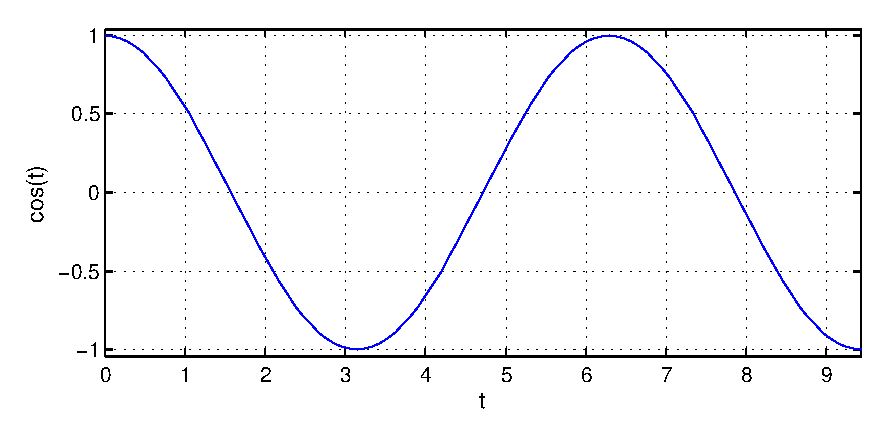
\includegraphics[width=0.495\textwidth]{\pwd/plots/example1}\label{fig:intro:floats:usage:figure-ex1}} \hfill
  \subfigure[right side]{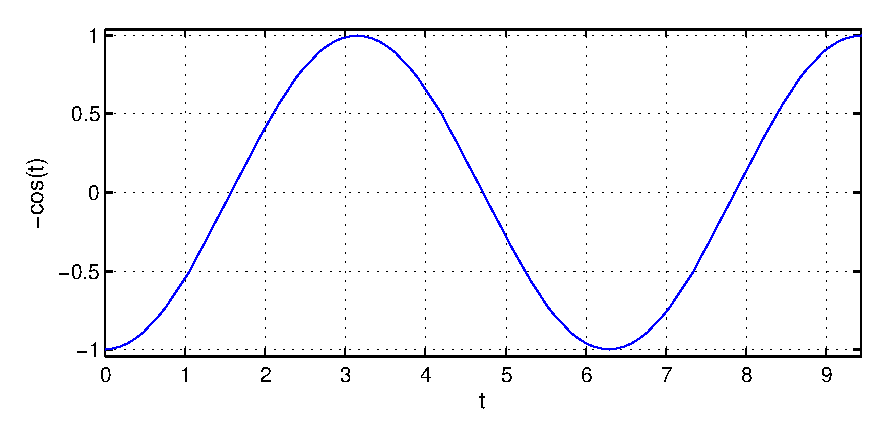
\includegraphics[width=0.495\textwidth]{\pwd/plots/example2}\label{fig:intro:floats:usage:figure-ex2}}
  \caption{Two subplots.}
  \label{fig:intro:floats:usage:figure}
\end{figure}

\noindent The same image can be created via a standardized command,
{\tiny\begin{verbatim}
  \twofigs{\pwd/plots/example1}{left side}{-ex1}{\pwd/plots/example2}{right side}{-ex2}{Two subplots.}{intro:floats:usage:figure-std}
\end{verbatim}}
\noindent and referenced like this: Fig.~\ref{fig:intro:floats:usage:figure-std}. There are several more standardized functions for figures, cf. Table~\ref{tab:intro:floats:figures}. Captions and labels are mandatory for all these commands.
\begin{longtable}{>{\tiny}l|>{\tiny}p{0.3\textwidth}}
  \normalsize\textbf{Command} & \normalsize\textbf{Description} \\\hline
  \verb|\fig{file}{caption}{label}| & Standard figure, full textwidth. \\\hline
  \verb|\figc{param}{file}{caption}{label}| & Standard figure with controllable parameters for includegraphics. \\\hline
  \verb|\twofig{file_l}{caption_l}{file_r}{caption_r}{caption}{label}| & Two figures, side by side. \\\hline
  \verb|\twofigs{file_l}{caption_l}{add.label_l}{filename_r}{caption_r}{add.label_l}{caption}{label}| & Two figures, side by side, with labels for each subfigure. Figure~\ref{fig:intro:floats:usage:figure-std} is created by this command.\\\hline
  \verb|\twofigc{param_l}{file_l}{caption_l}{param_l}{filename_r}{caption_r}{caption}{label}| & Two figures, side by side, with controllable parameters for includegraphics. \\\hline
  \verb|\figf|, \verb|\figcf|, \verb|\twofigf|, \verb|\twofigsf|, \verb|\twofigcf| & Like the above, but with framed figures. \\
  \caption{Standardized commands for figures.}
  \label{tab:intro:floats:figures}
\end{longtable}

\twofigs{\pwd/plots/example1}{left side}{-ex1}{\pwd/plots/example2}{right side}{-ex2}{Two subplots.}{intro:floats:usage:figure-std}



% **************************************************************************************************
\newsubsection{Listings}{intro:floats:listings}

\filelisting{matlab}{\pwd/plots/matlab.m}{Some matlab code example (highlighting can be configured).}{code-example}
% **************************************************************************************************
% **************************************************************************************************
\newsection{Miscellaneous}{intro:misc}

The template also provides several commands that make life easier. The ``reminder'' commands, for example, can be used to \reminder{mark something that should be revised}, but also as a placeholder for leftout parts of a \rem, if there is some open question \remq, or you have to look up some reference \remc. They can easily be found in the source code: Just search for \verb|\rem|. A second group of commands is used to create nice value-unit pairs, such as \vu{f=3}{kHz}, \vuc{2}{\textmu V}{\pm1}, or \vum{T\leq735}{\textdegree}{\pm4}. Feel free to redefine them to your needs.

\nxtpar\noindent
Oh, by the way: This section is \uc








% chapter 2
%    \emptydoublepage %FOR THESIS: ALWAYS START CHAPTERS AT RIGHT SIDE
\newchapter{Fancy and Advanced}{advanced}
\renewcommand{\pwd}{chapter2}
% **************************************************************************************************
% **************************************************************************************************
\newsection{Bringing Style Into Your Thesis}{fancy:style}
\openingquote{They misunderestimated me.}{Guess Who}

The template does not provide too many ``stylish'' commands. One of them created the quote above, the others are intended to mark a part of the text using the margins. You can, for example

\bigskip\bigskip
\dots state that this is dangerous.\MDanger

\bigskip\bigskip
\dots tell the reader to ``better pay attention''.\MAttention

\bigskip\bigskip
\dots mark some central results.\MHint

\bigskip\bigskip
\dots also admit that you're just clueless.\MQuestion








% **************************************************************************************************
% **************************************************************************************************
\newsection{Higher Mathematics}{fancy:math}

Naturally, there are also several commands that should make life easier when dealing with equations. One of the central ideas is to be able to change the general style of something, for example vector/matrix highlighting ($\vm{\phi}$ vs. $\phi$), just by modifying the template command.

\nxtpar\noindent
Here are a few examples. Note that equations (\ref{eq:fancy:math:1}) and (\ref{eq:fancy:math:2}), but also (\ref{eq:fancy:math:3a}) and (\ref{eq:fancy:math:3b}) do not necessarily make sense...
\begin{equation}
  \var{a + b} \isreq \var{a} + \var{b} + 2 \cov{a,b}
  \label{eq:fancy:math:1}
\end{equation}
\begin{equation}\begin{split}
  \vm{H}
  &\isdef \exp{\E{\vm{h}^T \vm{h}}} - \ln{\vm{h}^T \vm{h}} + \log{\vm{h}^T \vm{h}} - \frac{\ld{\vm{h}^T \vm{h}}}{\logb{3}{\vm{h}^T \vm{h}}} \\
  &= \mtx{ccc}{h1 & h2 & \dots \\ 0 & h1 & \dots \\ \vdots & \vdots & \ddots}
  \label{eq:fancy:math:2}
\end{split}\end{equation}
\begin{align}
  \E{ a b\conj c d\conj} &= \E{a b\conj} \cdot \E{c d\conj} + \E{a d\conj} \cdot \E{c b\conj} \label{eq:fancy:math:3a}\\
   \E{a b\conj} \cdot \E{c d\conj} &\neq  \E{a d\conj} \cdot \E{c b\conj} - \E{ a b\conj c d\conj}\label{eq:fancy:math:3b}
\end{align}



% **************************************************************************************************
%\appendix
% \bibliographystyle{./base/IEEEtran}
% \bibliography{_bibliography}


% **************************************************************************************************
% **************************************************************************************************

% place all floats and create label on last page
\FloatBarrier\label{end-of-document}
\end{document}

